\documentclass[a4paper, 12pt]{extarticle}

\usepackage{xecyr}
\usepackage{color}
\usepackage{float}
\usepackage{fontenc}
\usepackage{amsmath}
\usepackage{xltxtra}
\usepackage{graphicx}
\usepackage{csquotes}
\usepackage{listings}
\usepackage{longtable}
\usepackage{indentfirst}
\usepackage{unicode-math}
\usepackage{subfig}
\usepackage[english, russian]{babel}
\usepackage[width=1.2\textwidth]{caption}

\usepackage{tikz}
\usetikzlibrary{arrows, shapes, positioning, shadows, trees}
\tikzset{
  basic/.style  = {draw, text width=4cm, drop shadow, font=\sffamily, rectangle},
  root/.style   = {basic, rounded corners=2pt, thin, align=center, fill=gray!1},
  level 1/.style = {basic, rounded corners=2pt, thin, align=center, fill=gray!1,
                    sibling distance=55mm, level distance=50pt,
                    edge from parent/.style={->,draw,fill=black},
                    >=latex},
  level 2/.style = {basic, rounded corners=2pt, thin, align=center, fill=gray!1,
                    sibling distance=55mm, level distance=50pt,
                    edge from parent/.style={->,draw,fill=black},
                    >=latex},
  level 3/.style = {basic, rounded corners=2pt, thin, align=center, fill=gray!1,
                    sibling distance=55mm, level distance=75pt,
                    edge from parent/.style={->,draw,fill=black},
                    >=latex, text width=5cm},
  level 4/.style = {basic, rounded corners=2pt, thin, align=center, fill=gray!1,
                    sibling distance=40mm, level distance=50pt,
                    edge from parent/.style={->,draw,fill=black},
                    >=latex, text width=3cm},
}


\usepackage{titlesec}
\titleformat{\section}
  {\normalfont\fontsize{14}{15}\bfseries}{\thesection}{5pt}{}
\titleformat{\subsection}
  {\normalfont\fontsize{14}{15}\bfseries}{\thesubsection}{5pt}{}
\titleformat{\subsubsection}
  {\normalfont\fontsize{14}{15}\bfseries}{\thesubsubsection}{5pt}{}

\usepackage{fontspec}
\defaultfontfeatures{Ligatures=TeX}
\setmainfont[Ligatures=TeX]{Times New Roman}

\usepackage[a4paper,margin=1in,heightrounded]{geometry}
\geometry{left=3cm}
\geometry{right=1.5cm}
\geometry{top=2cm}
\geometry{bottom=2cm}

\usepackage{expl3}
\ExplSyntaxOn
\cs_new_eq:NN \Repeat \prg_replicate:nn
\ExplSyntaxOff

\usepackage[maxnames=5,
				backend=bibtex,
        %backend=biber,
				%style=gost-numeric,
        sorting=none,
				autolang=other]{biblatex}
\addbibresource{bibliography}


% Sections style redefinition
\renewcommand{\thesection}
  {\thepart\arabic{section}.}
\renewcommand{\thesubsection}
  {\thepart\arabic{section}.\arabic{subsection}.}
\renewcommand{\thesubsubsection}
  {\thepart\arabic{section}.\arabic{subsection}.\arabic{subsubsection}.}

% Equations, fugures, tables numbering style redefinition
\renewcommand{\theequation}
  {\thesection\arabic{equation}}
\renewcommand{\thefigure}
  {\thesection\arabic{figure}}
\renewcommand{\thetable}
  {\thesection\arabic{table}}

% Enum style redefinition
\renewcommand{\labelenumii}
  {\labelenumi\arabic{enumii}.}
\renewcommand{\labelenumiii}
  {\labelenumii\arabic{enumiii}.}

% Enlarge table row height
\renewcommand{\arraystretch}{1.2}

% Font to inline code highlighting
% Consolas must be installed!!!
\newfontfamily{\codefont}[Scale=0.9]{Consolas}
\newfontfamily{\listingsfont}[Scale=1.0]{Consolas}

% Define default style for codelisitngs
\definecolor{codegreen}{rgb}{0.00, 0.50, 0.00}
\definecolor{codegray} {rgb}{0.50, 0.50, 0.50}
\definecolor{codenumb} {rgb}{0.00, 0.00, 1.00}
\definecolor{codeblue} {rgb}{0.00, 0.43, 0.13}
\definecolor{codebrick}{rgb}{0.64, 0.08, 0.08}
\lstset{
  backgroundcolor=\color{white},
  basicstyle=\fontsize{10}{12}\selectfont\listingsfont,
  breakatwhitespace=false,
  breaklines=true,
  captionpos=b,
  commentstyle=\color{codegreen},
  frame=l,
  keepspaces=true,
  keywordstyle=\color{codeblue},
  language=C++,
  numbers=left,
  numbersep=8pt,
  numberstyle=\tiny\color{codegray},
  rulecolor=\color{black},
  showspaces=false,
  showstringspaces=false,
  showtabs=false,
  stepnumber=1,
  stringstyle=\color{codebrick},
  tabsize=2,
  title=\lstname
}

% Listing numbering style redefinition
\renewcommand{\lstlistingname}{Листинг}
\AtBeginDocument{
  \renewcommand{\thelstlisting}{\thesection\arabic{lstlisting}}
}

\newtheorem{hypothesis}{Гепотеза}

\DeclareMathOperator*{\argmax}{arg\,max}
\DeclareMathOperator*{\argmin}{arg\,min}
\DeclareMathOperator{\sign}{sign}

\begin{document}

\begingroup
\fontsize{14pt}{17pt}\selectfont
\begin{titlepage}

\begin{center}
МИНИСТЕРСТВО ОБРАЗОВАНИЯ И НАУКИ РОССИЙСКОЙ ФЕДЕРАЦИИ \\*
Федеральное   государственное  автономное  образовательное  учреждение \\*
высшего образования \\*
\textbf{<<Национальный исследовательский \\*
Нижегородский государственный университет им. Н.И. Лобачевского>> \\*
(ННГУ)}
\end{center}

\vspace{12pt}

\begin{center}
\textbf{Институт информационных технологий, математики и механики}
\end{center}

\begin{center}
\textbf{Кафедра: Математического обеспечения и суперкомпьютерных технологий}
\end{center}

\vspace{25pt}
\begin{center}
Направление подготовки: «Прикладная математика и информатика» \\*
Магистерская программа: «Системное программирование»
\end{center}
\vspace{30pt}

\begin{center}
\fontsize{18pt}{0pt}\textbf{ОТЧЁТ} \\*
по производственной практике
\end{center}
\begin{center}
на тему: \\*
\fontsize{16pt}{0pt}\textbf{<<Исследование методов учёта локальных свойств целевой функции в задачах глобальной оптимизации>>}
\end{center}

\vspace{53pt}

\begin{flushright}
\textbf{Выполнил}: студент группы 381503м4 \\*
\Repeat{17}{\_} Соврасов В.В. \\*
Подпись \Repeat{32}{\ } \\*

\textbf{Научный руководитель}: \Repeat{19}{\ } \\*
доцент, к.ф.м.н. \Repeat{34}{\ } \\*
\Repeat{17}{\_} Баркалов К.А. \\*
Подпись \Repeat{32}{\ }
\end{flushright}

\vspace{\fill}

\begin{center}
Нижний Новгород \\*
2016
\end{center}

\end{titlepage}
 % Link to main page
\endgroup

\begingroup
\fontsize{12pt}{20pt}\selectfont

\newpage
\thispagestyle{empty}
\tableofcontents

\newpage
\setcounter{page}{1}
\section{Введение}
Задачи нелинейной глобальной оптимизации встречаются в различных прикладных областях и традиционно считаются одними из самых трудоёмких среди оптимизационных задач.
Их сложность экспоненциально растёт в зависимости от размерности пространства поиска, поэтому для решения существенно многомерных задач требуются
суперкомпьютерные вычисления.
\par
В настоящее время на кафедре МОиСТ активно ведётся разработка программной системы для глобальной оптимизации функций многих вещественных переменных ExaMin.
Эта система включает в себя последние теоретические разработки, сделанные на кафедре в этой сфере, в том числе и блочную многошаговую схему редукции размерности \cite{blockNested}.
Отличительной чертой ситемы является то, что, она может работать как на CPU, так на разных типах ускорителей вычислений с высокой степенью параллельности (Xeonvarphi, GPU Nvidia) \cite{examinArtcle, examinphiArtcle}.
\par
В данной работе будут описаны некеторые улучшения, внесённые в систему, и предварительные исследования, проведённые перед их внедрением.
\section{Постановка задачи глобальной липшицевой оптимизации}
Одна из постановок задачи глобальной оптимизации звучит следующим образом: найти глобальный минимум \(N\)-мерной функции \(\varphi(y)\) в гиперинтервале \(D=\{y\in R^N:a_i\leqslant x_i\leqslant{b_i}, 1\leqslant{i}\leqslant{N}\}\).
Для построения оценки глобального минимума по конечному количеству вычислений значения функции требуется, чтобы \(\varphi(y)\) удовлетворяла условию Липшица.
\begin{displaymath}
\label{task}
\varphi(y^*)=\min\{\varphi(y):y\in D\}
\end{displaymath}
\begin{displaymath}
\label{lip}
|\varphi(y_1)-\varphi(y_2)|\leqslant L\Vert y_1-y_2\Vert,y_1,y_2\in D,0<L<\infty
\end{displaymath}
\par
Классической схемой редукции размерности для алгоритмов глобальной оптимизации является использование разверток --- кривых, заполняющих пространство \cite{strOptBook}.
\begin{displaymath}
\label{cube}
\lbrace y\in R^N:-2^{-1}\leqslant y_i\leqslant 2^{-1},1\leqslant i\leqslant N\rbrace=\{y(x):0\leqslant x\leqslant 1\}
\end{displaymath}
\par
 Такое отображение позволяет свести задачу в многомерном пространстве к решению одномерной ценой ухудшения её свойств. В частности, одномерная функция \(\varphi(y(x))\) является не
 Липшицевой, а Гёльдеровой:
\begin{displaymath}
\label{holder}
|\varphi(y(x_1))-\varphi(y(x_2))|\leqslant H{|x_1-x_2|}^{\frac{1}{N}},x_1,x_2\in[0,1]
\end{displaymath}
где константа Гельдера \(H\) связана с константой Липшица \(L\) соотношением
\begin{displaymath}
H=4Ld\sqrt{N},d=\max\{b_i-a_i:1\leqslant i\leqslant N\}
\end{displaymath}
\par
\section{Алгоритм глобального поиска}
 Для дальнейшего изложения потребуется описание метода глобальной оптимизации, используемого в системе ExaMin. Многомерные задачи сводятся к одномерным с помощью различных схем редукции размерноти,
 поэтому можно рассматривать минимизацию одномерной функции  \(f(x), x\in[0,1]\), удовлетворяющей условию Гёльдера.
\par
Рассматриваемый алгоритм решения данной задачи предполагает построение последовательности точек \(x_k\), в которых вычисляются значения минимизируемой функции \(z_k = f(x_k)\).
Процесс вычисления значения функции (включающий в себя построение образа \(y_k=y(x_k))\) будем называть испытанием, а пару \((x_k,z_k)\) --- результатом испытания.
Множество пар \(\{(x_k,z_k)\}, 1\leqslant k\leqslant n\) составляет поисковую информацию, накопленную методом после проведения \(n\) шагов.
\par
На первой итерации метода испытание проводится в произвольной внутренней точке \(x_1\) интервала \([0;1]\). Пусть выполнено \(k\geqslant 1\) итераций метода,
в процессе которых были проведены испытания в \(k\) точках \(x_i, 1\leqslant i\leqslant k\). Тогда точкa \(x^{k+1}\) поисковых испытаний следующей \((k+1)\)-ой
итерации определяются в соответствии с правилами:
\par
Шаг 1. Перенумеровать точки множества \(X_k=\{x^1,\dotsc,x^k\}\cup\{0\}\cup\{1\}\), которое включает в себя граничные точки интервала \([0,1]\), а также точки предшествующих испытаний, нижними индексами в порядке увеличения значений координаты, т.е.
\begin{displaymath}
0=x_0<x_1<\dotsc<x_{k+1}=1
\end{displaymath}
\par
Шаг 2. Полагая \(z_i=f(x_i),1\leqslant i\leqslant k\), вычислить величины
\begin{equation}
\label{step2}
\mu=\max_{1\leqslant i\leqslant k}\dfrac{|z_i-z_{i-1}|}{\Delta_i},
\begin{matrix}
    M =
    \left\{
    \begin{matrix}
    r\mu,\mu>0 \\
    1,\mu=0
    \end{matrix} \right.
    \end{matrix}
\end{equation}
где \(r\) является заданным параметром метода, а \(\Delta_i=(x_i-x_{i-1})^\frac{1}{N}\).
\par
Шаг 3. Для каждого интервала \((x_{i-1},x_i),1\leqslant i\leqslant k+1\), вычислить характеристику в соответствии с формулами
\begin{equation}
\label{step3_1}
R(1)=2\Delta_1-4\dfrac{z_1}{M},R(k+1)=2\Delta_{k+1}-4\dfrac{z_k}{M}
\end{equation}
\begin{equation}
\label{step3_2}
R(i)=\Delta_i+\dfrac{(z_i-z_{i-1})^2}{M^2\Delta_i}-2\dfrac{z_i+z_{i-1}}{M},1<i<k+1
\end{equation}
\par
Шаг 4. Выбрать наибольшую характеристику:
\begin{equation}
\label{step4}
t=\argmax_{1\leqslant i \leqslant k+1}R(i)
\end{equation}
\par
Шаг 5. Провести очередное испытания в точке \(x_{k+1}\), вычисленной по формулам
\begin{displaymath}
x_{k+1}=\dfrac{x_{t}+x_{t-1}}{2},t=1,t=k+1
\end{displaymath}
\begin{equation}
\label{step5}
x_{k+1}=\dfrac{x_{t}+x_{t-1}}{2}-\sign(z_{t}-z_{t-1})\dfrac{1}{2r}\left[\dfrac{|z_{t}-z_{t-1}|}{\mu}\right]^N,1<t<k+1
\end{equation}
\par
Алгоритм прекращает работу, если выполняется условие \(\Delta_{t}\leqslant \varepsilon\), где \(\varepsilon>0\) есть заданная точность. В качестве оценки глобально-оптимального решения задачи  выбираются значения
\begin{equation}
f_k^*=\min_{1\leqslant i \leqslant k}f(x_i), x_k^*=\argmin_{1\leqslant i \leqslant k}f(x_i)
\end{equation}
\par
Подробнее метод и теорема о его сходимости описаны в \cite{strOptBook}.
\subsection{Сравнение методов оптимизации} \label{subsec:methods_compasion}
Существует несколько критериев оптимальности алгоритмов поиска (минимаксный, критерий одношаговой оптимальности), но большинстве случаев представляет интерес
сравнение методов по среднему результату, достижимому на конкретном подклассе липшицевых функций. Достоинством такого подхода является то, что средний показатель можно оценить
по конечной случайной выборке задач, используя методы математической статистики.
\par
В качестве оценки эффективности алгоритма будем использовать, операционную характеристику, которая определяется множеством точек на плоскости \((K, P)\),
где \(K\) – среднее число поисковых испытаний, предшествующих выполнению условия остановки при минимизации функции из данного класса, а \(P\) – статистическая вероятность того,
что к моменту остановки глобальный экстремум будет найден с заданной точностью. Если при выбранном \(K\) операционная характеристика одного метода лежит выше характеристики другого,
то это значит, что при фиксированных затратах на поиск первый метод найдёт решение с большей статистической вероятностью. Если же зафиксировать некоторое значение \(P\), и
характеристика одного метода лежит левее характеристики другого, то первый метод требует меньше затрат на достижение той же надёжности.
\subsection{Классы тестовых задач} \label{subsec:test_problems}
Для сравнения алгоритмов глобального поиска в смысле операционной характеристики требуется иметь некоторое множество тестовых задач.
Генератор задач GKLS, описанный в \cite{gklsBook} позволяет получить такое множество задач с заренее известными свойствами.
В данной работе используются два класса, сгенерированные GKLS: 4d Simple и 5d Simple, параметры которых также описаны в \cite{gklsBook}. Функции рассматриваемых классов являются непрерывно
дифференцируемыми и имеют 10 локальных минимумов, один из которых является глобальным.

\section{Применение локальных оценок константы Гёльдера для ускорения сходимости АГП}
Как видно из описания метода, независимо от локальных свойств оптимизируемой одномерной
функции, для вычисления характеристик всех интервалов (\ref{step3_1}), (\ref{step3_2}) используется одно и то же
значение оценки константы Гёльдера (\ref{step2}). В работе \cite{sergLocalTuningFirst} было предложено использовать различные
значения \(M\) (\(M\) из (\ref{step2}), (\ref{step3_1})) для каждого интревала, а
также показана эффективность такого подхода в случае одномерной оптимизации функций,
удовлетворяющих условию Липшица. В работе \cite{nestedLocal} рассмотрено применение
адаптивных оценок констант Липшица в схеме многомерной вложенной оптимизации.

Для каждого интревала локальная оценка константы является максимум-аддитивной свёрткой
<<глобальной>> и <<локальной>> компонент (\(\gamma\) и \(\lambda\) соответственно):
\begin{displaymath}
  \begin{array}{lr}
    \lambda_i=\max\{H_{i-1},H_i,H_{i+1}\} \\
    H_i=\frac{|z_i-z_{i-1}|}{\Delta_i} \\
    H^k=\max\{H_i:i=2,\dots ,k\} \\
    \gamma_i=H^k\frac{\Delta_i}{\Delta^{max}} \\
    \Delta^{max}=\max\{\Delta_{i}:i=2,\dots ,k\}
  \end{array}
\end{displaymath}
\begin{equation}
\label{additiveConv}
M_i=r\cdot \max\{H_i, \frac{1}{2}(\lambda_i+\gamma_i),\xi\}
\end{equation}

Параметр \(\xi\) предотвращает обнуление оценки \(M_i\) в случае, если оптимизируемая
фнкция является тождественной константой, и выбирается достаточно малым.
Данный вариант свёртки не зависит от параметра \(r\), однако в \cite{sergLocalTuning}
также рассматриваетсяи адаптивная свёртка:
\begin{equation}
\label{additiveAdaptiveConv}
M_i=r\cdot \max\{H_i, \frac{\lambda_i}{r}+\frac{r-1}{r}\gamma_i,\xi\}
\end{equation}

Если априори известно, что оптимизируемая функция имеет сложный рельеф с множеством
локальных минимумов, то \(r\) изначально задаётся большим, что ведёт к преобладанию в
адаптивной свёртке «глобальной» сооставляющей \(\gamma\).

Оба варианта свёртки (\ref{additiveConv}), (\ref{additiveAdaptiveConv}) были предложены
и детально рассмотрены в \cite{sergLocalTuning} для случая одномерных функций,
удовлетворяющих условию Липшица. В данном разделе будет рассмотрено применение этих
свёрток для оптимизации двумерных функций в случае редукции размерности с помощью развёрток.

В \cite{sergLocalTuning} приведена теорема о сходимости метода в случае, если целевая функция
липшицева, однако, как правило, подобные утверждения справедливы и в Гёльдеровой метрике, поэтому,
предположительно, будет верна следующая гепотеза:
\begin{hypothesis}
Пусть целевая функция \(f(x)\) удовлетвворяет условию Гёльдера с конечной константой
\(H > 0\), и пусть \(x\) является предельной точкой последовательности \(\{x_k\}\),
порождаемой алгоритмом. Тогда верны следующие утверждения:
\begin{enumerate}
  \item Если \(x\in(0;1)\), то сходимость к точке \(x\) является двухсторонней, т.е.
  существуют две подпоследовательности \(\{x_k\}\), сходящиеся к \(x\): одна слева,
  а другая справа;
  \item \(f(x_k) \geqslant f(x)\) для всех точек испытаний \(x_k, k \geqslant 1\);
  \item Если существует другая предельна точка \(x^* = x\), то \(f(x) = f(x^*)\);
  \item Если функция \(f(x)\) имеет конечное число локальных минимумов на отрезке \([0, 1]\),
  то точка \(x\) является локально оптимальной;
  \item (Существенное условие сходимости к глобальномк минимуму). Пусть \(x^*\)
  является глобальным минимумом \(f(x)\). Если существует такое число \(k^*\),
  что для всех итераций с номерами \(k > k^*\) неравенство
  \(M_j(k) > H_j(k)\) выполняется, где \(H_j(k)\) --- это константа Гёльдера на интервале
  \([x_{j(k)-1}, x_{j(k)}]\), содержащем \(x^*\), а \(M_{j(k)}\) её оценка.
  Тогда множество предельных точек последовательности \(\{x_k\}\) совпадает с множеством
  глобальных минимумов функции \(f(x)\).
\end{enumerate}
\end{hypothesis}

Доказательство гепотезы требует отдельных теоретических исследований. В рамках данной
работы оно не будет проведено, наличие сходимости установлено только численно.

Эксперименты по оценке эффективности метода с локально-адаптивной оценкой константы
Гёльдера производились на двумерных классах задач Гришагина (\(F_{GR}\))
и GKLS Simple 2d, упомянутых в разделе \ref{subsec:test_problems}
Каждый из классов содержит 100 многоэкстремальных функций. Развёртка во всех экспериментах
строилась с плотностью \(m=12\), параметр \(\varepsilon\) в критерии остановки был равен \(10^{-3}\).
Параметр \(r\) выбирался минимально возможным, при котором заданный метод решает все
задачи класса. Шаг поиска \(r\) равен \(0.1\).

\begin{figure}[ht]
    \centering
    \subfloat[глобальная оценка \(H\)]{{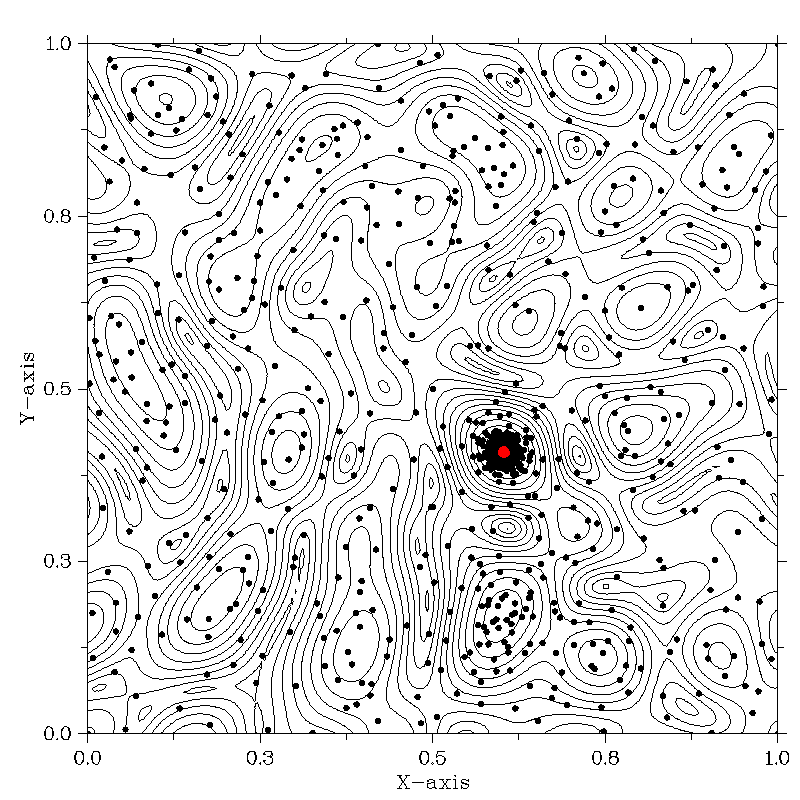
\includegraphics[width=0.45\textwidth]{images/gs_glob.png} }}
    \qquad
    \subfloat[локально-адаптивная оценка \(H\)]{{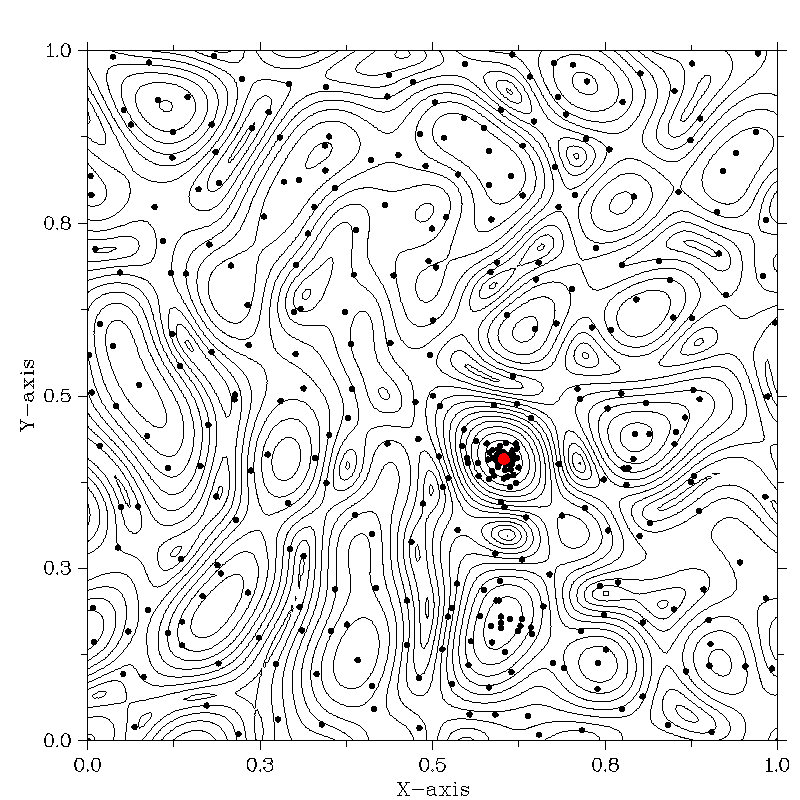
\includegraphics[width=0.45\textwidth]{images/gs_loc.png} }}
    \caption{Линии уровня одной из функций класса \(F_{GR}\)}
    \label{fig:grish_isolines}
\end{figure}

Для наглядной иллюстрации преимущества локально-адаптивной схемы оценки константы
\(H\) рассмотрим результаты работы метода на конкретном примере. На рис. \ref{fig:grish_isolines} показаны
линии уровня одной из функций класса \(F_{GR}\) и точки испытаний, проведённых методом с глобальной
оценкой константы Гёльдера и с оценкой по формуле (\ref{additiveConv}). Как видно из рисунков, метод с
глобальной оценкой константы проводит большое число испытаний в окрестности точки
глобального минимума прежде (всего проведено 1086 испытаний), чем выполнится условие
остановки, в то врямя, как метод с локально-адаптивной оценкой гораздо быстрее
сходится (всего проведено 385 испытаний). Аналогичная ситуация имеет место при
оптимизации одной из функций класса GKLS Simple 2d (рис. \ref{fig:gkls_isolines}). Метод с глобальной
оценкой константы произвёл 2600 испытаний, а метод с локально-адаптивной оценкой – 1190.

\begin{figure}[ht]
    \centering
    \subfloat[глобальная оценка \(H\)]{{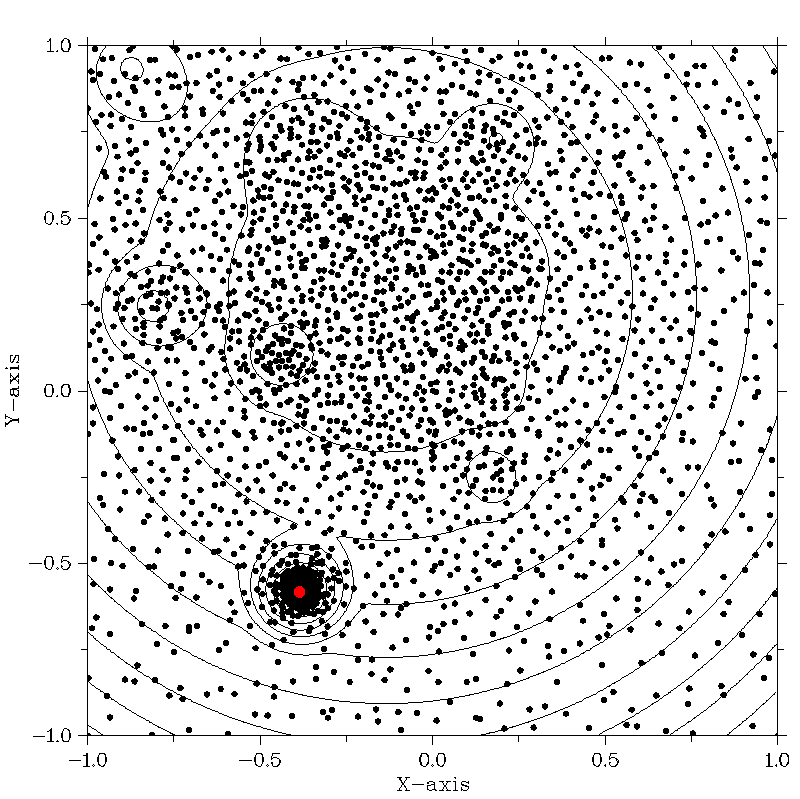
\includegraphics[width=0.45\textwidth]{images/gkls_glob.png} }}
    \qquad
    \subfloat[локально-адаптивная оценка \(H\)]{{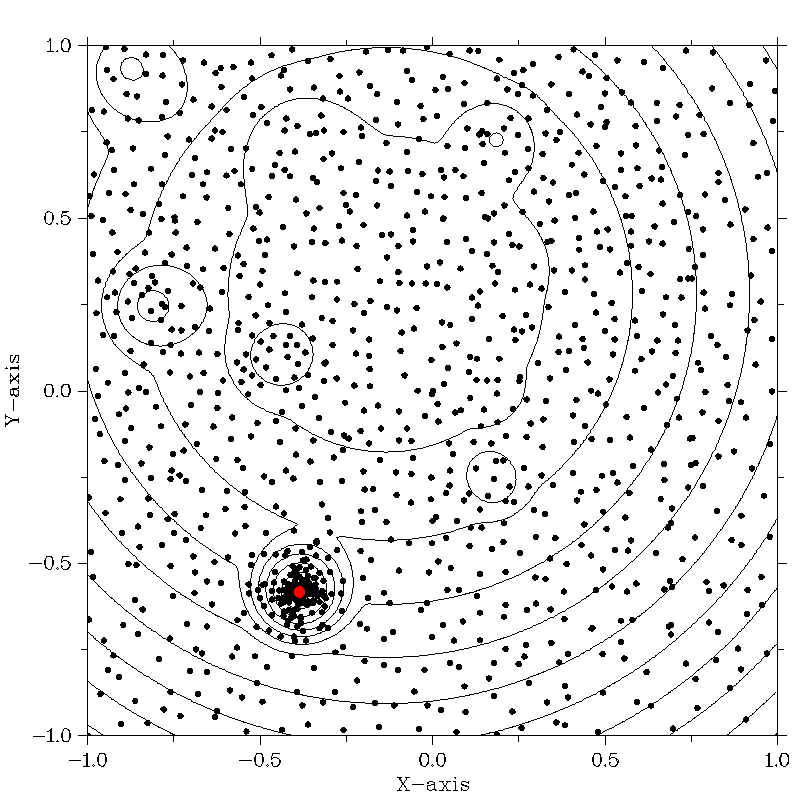
\includegraphics[width=0.45\textwidth]{images/gkls_loc.png} }}
    \caption{Линии уровня одной из функций класса GKLS Simple 2d}
    \label{fig:gkls_isolines}
\end{figure}

\begin{figure}[ht]
  	\center
    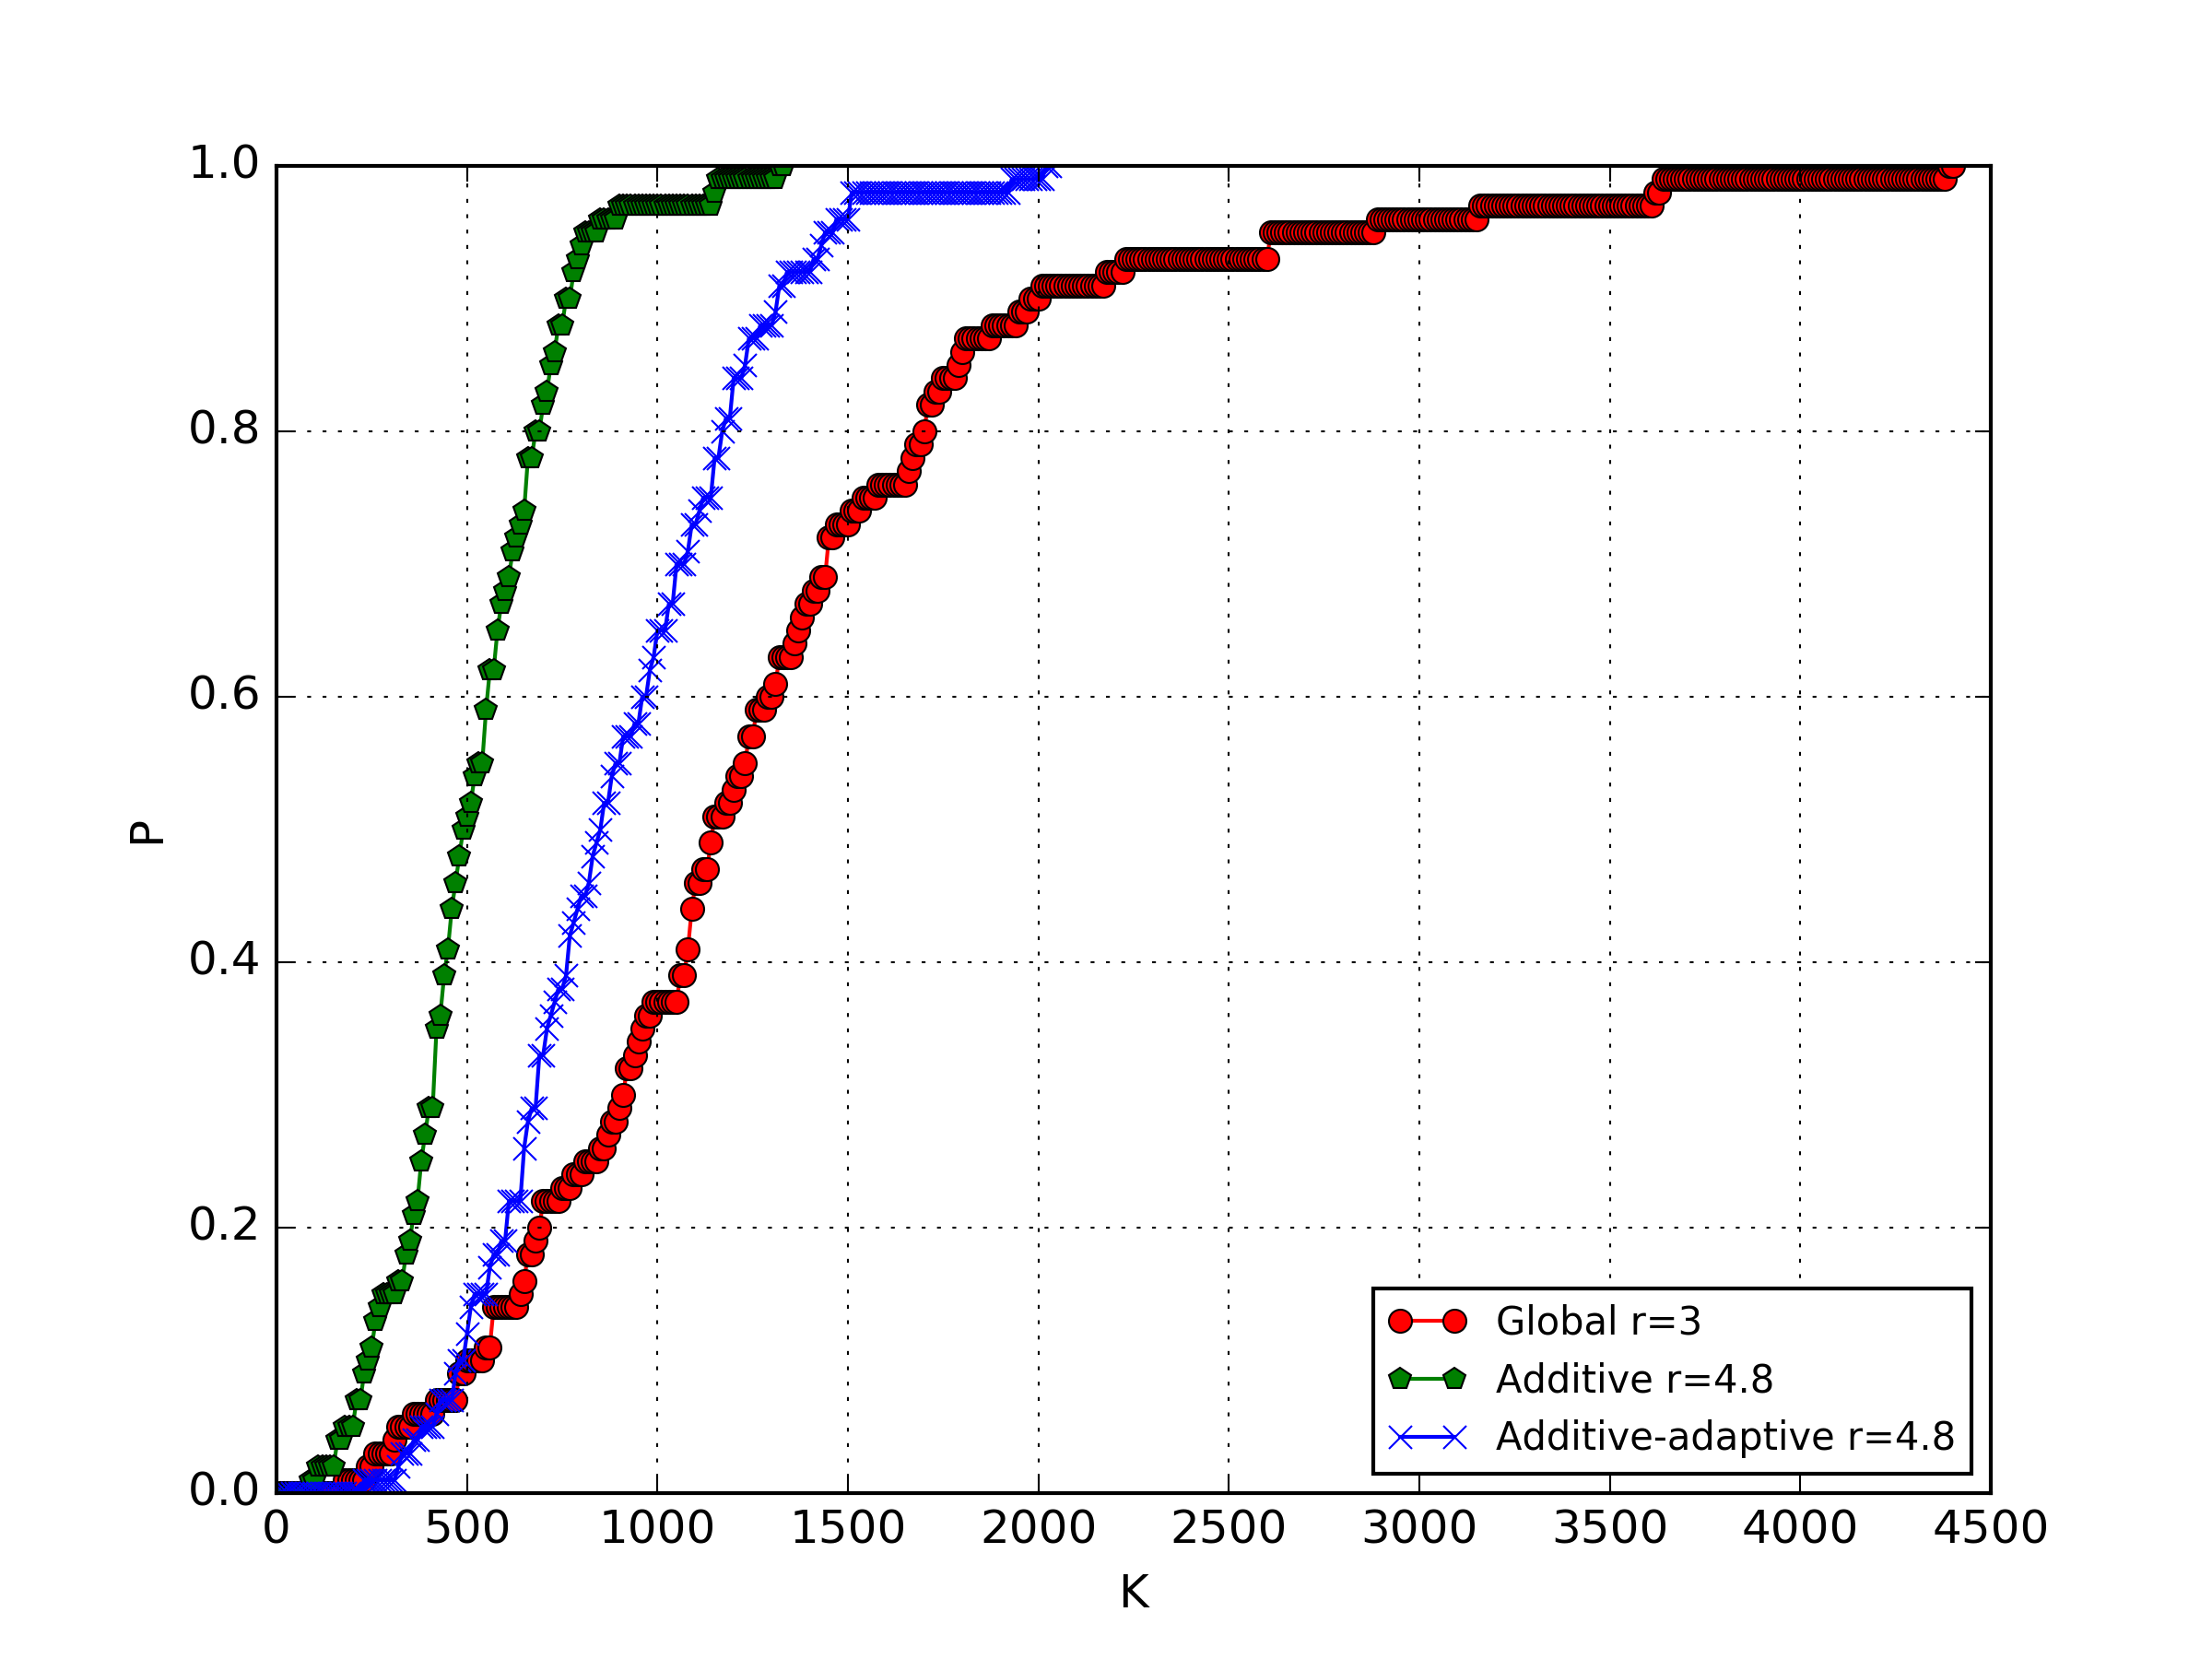
\includegraphics[width=0.75\textwidth]{images/grishagin.png}
    \caption{Операционные характеристики методов на классе задач \(F_{GR}\)}
    \label{fig:grishh_op}
\end{figure}

\begin{figure}[H]
  \center
  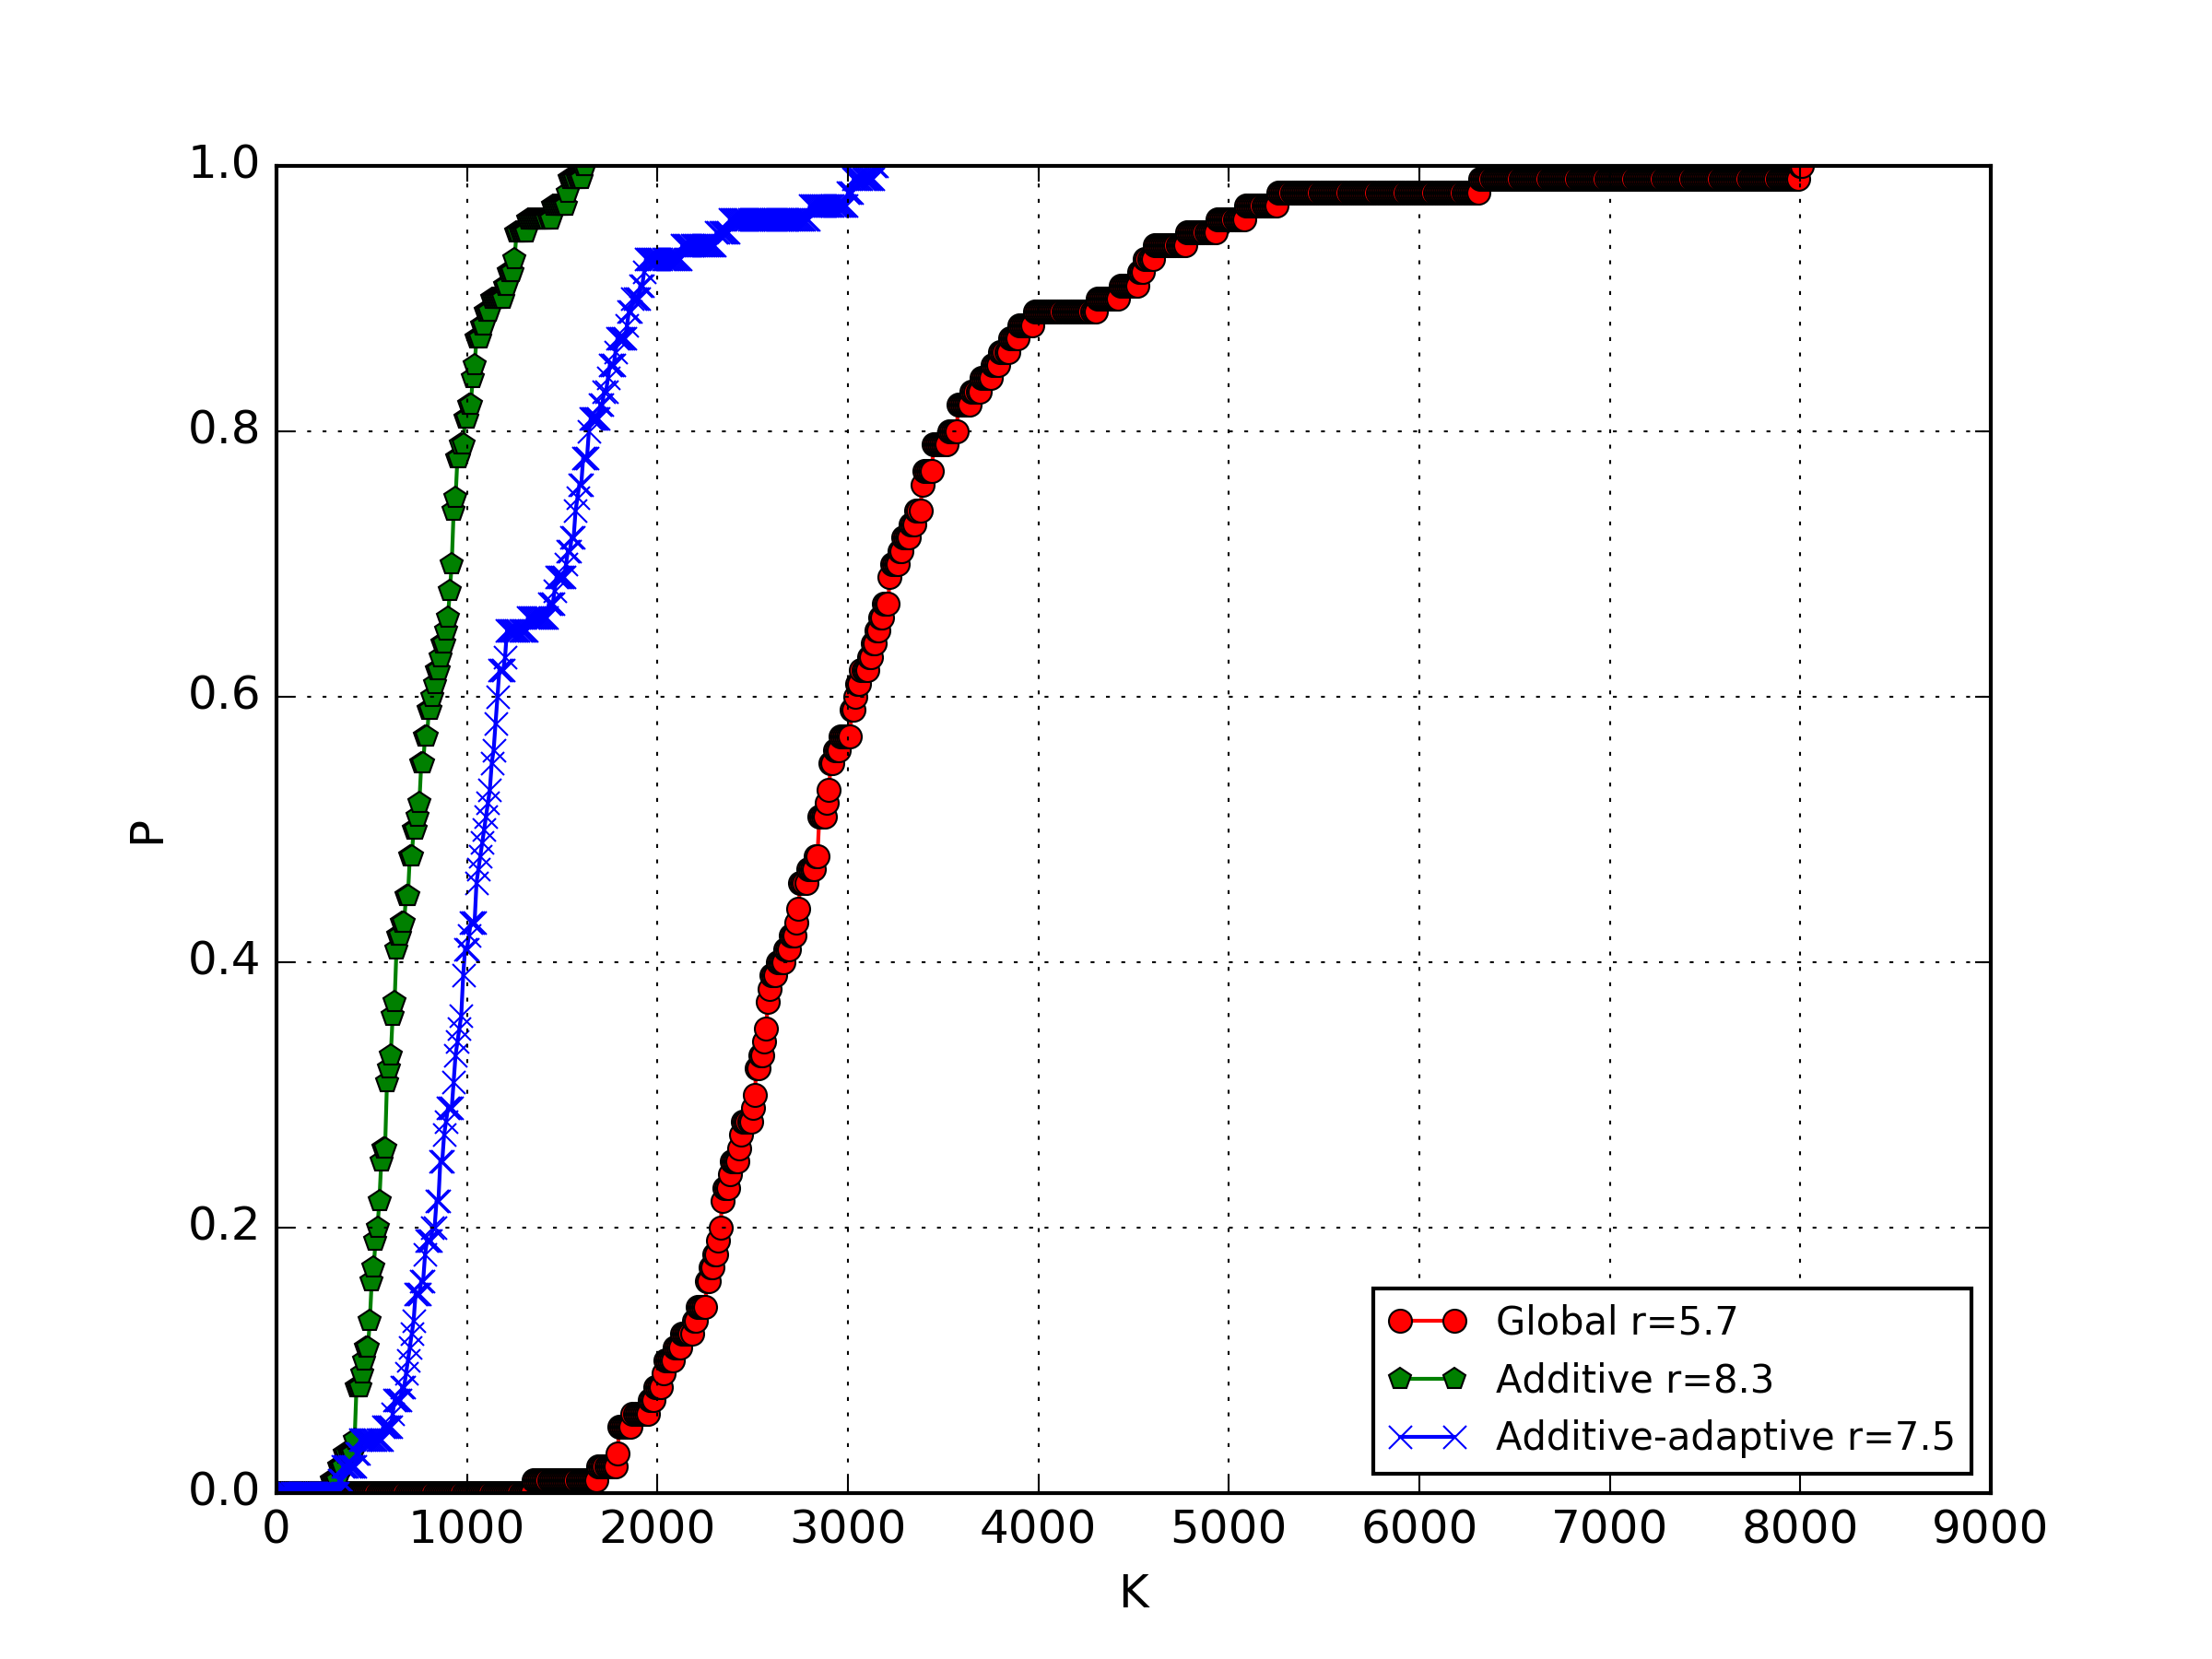
\includegraphics[width=0.75\textwidth]{images/gkls-s.png}
  \caption{Операционные характеристики методов на классе задач GKLS Simple 2d}
  \label{fig:gkls_op}
\end{figure}

Далее перейдём к сравнению различных вариантов метода на рассматриваемых классах задач.
В качестве оценки эффективности алгоритма будем использовать, операционную характеристику,
описанную в разделе \ref{subsec:methods_compasion}

Как видно из операционных характеристик на рис. \ref{fig:grishh_op} и \ref{fig:gkls_op},
оба метода с локально-адаптивной оценкой константы Гёльдера показали существенное преимущество, однако они требуют
задавать более высокое значение параметра \(r\). Если сравнивать между собой методы с
адаптивной и неадаптивной свёрткой (\ref{additiveConv}), (\ref{additiveAdaptiveConv}), то наглядно видно преимущество последнего,
хотя он и требует большее значение параметра надёжности \(r\) для решения задач из класса GKLS.

\section{Заключение}
В ходе работы были получены следующие практические результаты:
\begin{itemize}
  \item cхема была реализована на языке C++ с помощью библиотеки Eigen \cite{eigenLib}.
  Исходный код можно найти в приложении \ref{attach2}.
\end{itemize}


\newpage
%\nocite{*}
\addcontentsline{toc}{section}{Список литературы}
\printbibliography
\newpage
\section{Приложения}
\subsection{Приложение 1}
\label{attach1}

\begin{lstlisting}[frame=single]
#ifndef OPTIMIZER_ALGORITHM_UNCONSTRAINED_HPP
#define OPTIMIZER_ALGORITHM_UNCONSTRAINED_HPP

#include "OptimizerCoreGlobal.hpp"
#include "OptimizerTask.hpp"
#include "OptimizerSolution.hpp"
#include "OptimizerFunction.hpp"
#include "OptimizerDataStructures.hpp"
#include "OptimizerSolution.hpp"
#include "OptimizerResult.hpp"
#include "OptimizerSearchSequence.hpp"

#include <set>

namespace optimizercore
{

	class EXPORT_API OptimizerAlgorithmUnconstrained final
	{

	private:

		bool mLocalMixType;
		bool mIsAlgorithmMemoryAllocated;
		bool mIsParamsInitialized;
		bool mIsTaskInitialized;
		bool mNeedLocalVerification;

		int mNumberOfThreads;
		int mLocalStartIterationNumber;
		int mMaxNumberOfIterations;
		int mMapTightness;
		int mMethodDimension;
		int mAlpha;
		int mLocalMixParameter;
		int mMapType;

		OptimizerSpaceTransformation mSpaceTransform;
		OptimizerFunction *mTargetFunction;
		OptimizerFunctionPtr mTargetFunctionSmartPtr;

		OptimizerInterval *mIntervalsForTrials;
		std::set<OptimizerTrialPoint> mSearchInformationStorage;
		OptimizerTrialPoint mOptimumEvaluation, *mNextTrialsPoints;

		LocalTuningMode mLocalTuningMode;

		double mGlobalM, mZ, eps, r, mMaxIntervalNorm;
		double **mNextPoints;

		void AllocMem();
		void InitializeInformationStorage();
		void UpdateGlobalM(std::set<OptimizerTrialPoint>::iterator&);
		int UpdateRanks(bool isLocal);
		bool InsertNewTrials(int trailsNumber);
		OptimizerSolution DoLocalVerification(OptimizerSolution startPoint);

	public:
		OptimizerAlgorithmUnconstrained();
		~OptimizerAlgorithmUnconstrained();

		void SetTask(OptimizerFunctionPtr function,
			OptimizerSpaceTransformation spaceTransform);
		void SetThreadsNum(int num);
		void SetParameters(OptimizerParameters params);

		OptimizerResult StartOptimization(const double* xOpt,
			StopCriterionType stopType);

		double GetLipschitzConst() const;
		OptimizerSearchSequence GetSearchSequence() const;

	};
}
#endif
\end{lstlisting}
\begin{lstlisting}[frame=single]
	#include "OptimizerAlgorithmUnconstrained.hpp"
	#include "HookeJeevesLocalMethod.hpp"

	#include <cassert>
	#include <algorithm>

	using namespace optimizercore;
	using namespace optimizercore::utils;

	OptimizerAlgorithmUnconstrained::OptimizerAlgorithmUnconstrained()
	{
		mIsAlgorithmMemoryAllocated = false;

		mLocalStartIterationNumber = 1;
		mNumberOfThreads = 1;
		mMaxNumberOfIterations = 5000;
		mNextPoints = nullptr;
		mNextTrialsPoints = nullptr;
		mIntervalsForTrials = nullptr;
		r = 2;
		mLocalTuningMode = LocalTuningMode::None;

		mIsTaskInitialized = false;
		mIsParamsInitialized = false;
	}

	void OptimizerAlgorithmUnconstrained::SetTask(OptimizerFunctionPtr function,
		OptimizerSpaceTransformation spaceTransform)
	{
		assert(function);

		mTargetFunctionSmartPtr = function;
		mTargetFunction = function.get();
		mSpaceTransform = spaceTransform;

		mIsTaskInitialized = true;
	}

	OptimizerSearchSequence OptimizerAlgorithmUnconstrained::GetSearchSequence() const
	{
		return OptimizerSearchSequence(mSearchInformationStorage, mMethodDimension,
			static_cast<MapType> (mMapType), mMapTightness, mSpaceTransform);
	}

	double OptimizerAlgorithmUnconstrained::GetLipschitzConst() const
	{
		return mGlobalM;
	}

	void OptimizerAlgorithmUnconstrained::SetParameters(OptimizerParameters params)
	{
		assert(params.algDimention);
		assert(params.eps > 0);
		assert(params.localAlgStartIterationNumber > 0);
		assert(params.mapTightness > 5 && params.mapTightness <= 20);
		assert(params.maxIterationsNumber > 0);
		assert(params.localMixParameter >= 0 && params.localMixParameter <= 20);
		assert(params.r != nullptr);
		assert(params.numberOfThreads > 0);
		assert(params.reserves != nullptr);
		assert(params.numberOfMaps > 0);

		mLocalStartIterationNumber = params.localAlgStartIterationNumber;
		eps = params.eps;
		if (params.localMixParameter <= 10)	{
			mLocalMixParameter = params.localMixParameter;
			mLocalMixType = true;
		}
		else	{
			mLocalMixParameter = 20 - params.localMixParameter;
			mLocalMixType = false;
		}
		mNeedLocalVerification = params.localVerification;
		mAlpha = params.localExponent;
		mMethodDimension = params.algDimention;
		mMapTightness = params.mapTightness;
		mMapType = static_cast<int>(params.mapType);
		mMaxNumberOfIterations = params.maxIterationsNumber;
		mLocalTuningMode = params.localTuningMode;
		r = *params.r;
		if (mNextPoints)
			utils::DeleteMatrix(mNextPoints, mNumberOfThreads);
		mNextPoints = utils::AllocateMatrix<double>(mNumberOfThreads, mMethodDimension);
		this->SetThreadsNum(params.numberOfThreads);

		mIsParamsInitialized = true;
	}

	void OptimizerAlgorithmUnconstrained::InitializeInformationStorage()
	{
		if (!mIsAlgorithmMemoryAllocated){
			AllocMem();
			mIsAlgorithmMemoryAllocated = true;
		}

		mZ = HUGE_VAL;
		mGlobalM = 1;
		mMaxIntervalNorm = 0;

		mSearchInformationStorage.clear();

		mapd(0.0, mMapTightness, mNextPoints[0], mMethodDimension, mMapType);
		mSpaceTransform.Transform(mNextPoints[0], mNextPoints[0]);
		mSearchInformationStorage.emplace(0.0, mTargetFunction->Calculate(mNextPoints[0]), 0);

		mapd(1.0, mMapTightness, mNextPoints[0], mMethodDimension, mMapType);
		mSpaceTransform.Transform(mNextPoints[0], mNextPoints[0]);
		mSearchInformationStorage.emplace(1.0, mTargetFunction->Calculate(mNextPoints[0]), 0);
	}

	bool OptimizerAlgorithmUnconstrained::InsertNewTrials(int trailsNumber)
	{
		bool storageInsertionError;
		if (mMapType == 3)
		{
			int preimagesNumber = 0;
			double preimages[32];
			for (int i = 0; i < trailsNumber; i++)
			{
				invmad(mMapTightness, preimages, 32,
					&preimagesNumber, mNextPoints[i], mMethodDimension, 4);
				for (int k = 0; k < preimagesNumber; k++)
				{
					mNextTrialsPoints[i].x = preimages[k];
					auto insertionResult =
						mSearchInformationStorage.insert(mNextTrialsPoints[i]);

					if (!(storageInsertionError = insertionResult.second))
						break;

					UpdateGlobalM(insertionResult.first);
				}
			}
		}
		else
			for (int i = 0; i < trailsNumber; i++)
			{
				auto insertionResult =
					mSearchInformationStorage.insert(mNextTrialsPoints[i]);

				if (!(storageInsertionError = insertionResult.second))
					break;

				UpdateGlobalM(insertionResult.first);
			}
		return storageInsertionError;
	}

	OptimizerResult OptimizerAlgorithmUnconstrained::StartOptimization(
		const double* a, StopCriterionType stopType)
	{
		assert(mIsParamsInitialized && mIsTaskInitialized);
		assert(mSpaceTransform.GetDomainDimension() == mMethodDimension);

		InitializeInformationStorage();

		double *y;
		bool stop = false;
		int iterationsCount = 0,
			currentThrNum = 1, ranksUpdateErrCode;

		mNextTrialsPoints[0].x = 0.5;
		mapd(mNextTrialsPoints[0].x, mMapTightness, mNextPoints[0],
			mMethodDimension, mMapType);
		mSpaceTransform.Transform(mNextPoints[0], mNextPoints[0]);

		while (iterationsCount < mMaxNumberOfIterations && !stop)	{
			iterationsCount++;

	#pragma omp parallel for num_threads(currentThrNum)
			for (int i = 0; i < currentThrNum; i++)	{
				mNextTrialsPoints[i].val = mTargetFunction->Calculate(mNextPoints[i]);
				if (mMapType == 3)
					mSpaceTransform.InvertTransform(mNextPoints[i], mNextPoints[i]);
	#pragma omp critical
				if (mNextTrialsPoints[i].val < mZ)
					mZ = mNextTrialsPoints[i].val;
			}

			if (!InsertNewTrials(currentThrNum))
				break;

			if (iterationsCount >= mLocalStartIterationNumber)	{
				if (iterationsCount % (12 - mLocalMixParameter) == 0
					&& mLocalMixParameter > 0)
					ranksUpdateErrCode = UpdateRanks(mLocalMixType);
				else
					ranksUpdateErrCode = UpdateRanks(!mLocalMixType);
			}
			else
				ranksUpdateErrCode = UpdateRanks(false);

			if (iterationsCount >= mNumberOfThreads + 10)
				currentThrNum = mNumberOfThreads;

			for (int i = 0; i < currentThrNum && !stop; i++)	{
				OptimizerTrialPoint left = mIntervalsForTrials[i].left;
				OptimizerTrialPoint right = mIntervalsForTrials[i].right;

				mNextTrialsPoints[i].x = (left.x + right.x) / 2
					- sgn(right.val - left.val)*pow(fabs(right.val - left.val)
					/ mIntervalsForTrials[i].localM, mMethodDimension) / (2 * r);

				mapd(mNextTrialsPoints[i].x, mMapTightness, mNextPoints[i],
					mMethodDimension, mMapType);
				mSpaceTransform.Transform(mNextPoints[i], mNextPoints[i]);

				y = mNextPoints[i];

				if (stopType == StopCriterionType::OptimalPoint)	{
					if (NormNDimMax(y, a, mMethodDimension) < eps)	{
						stop = true;
						mOptimumEvaluation = mNextTrialsPoints[i];
					}
				}
				else	{
					if (pow(right.x - left.x, 1.0 / mMethodDimension) < eps)	{
						stop = true;
						mOptimumEvaluation = mNextTrialsPoints[i];
					}
				}
			}
		}

		mOptimumEvaluation.val = mTargetFunction->Calculate(y);
		mSearchInformationStorage.insert(mOptimumEvaluation);

		if (stopType == StopCriterionType::Precision)
			mOptimumEvaluation = *std::min_element(mSearchInformationStorage.begin(),
				mSearchInformationStorage.cend(),
				[](OptimizerTrialPoint p1, OptimizerTrialPoint p2)
			{
				return p1.val < p2.val;
			});

		mapd(mOptimumEvaluation.x, mMapTightness, y, mMethodDimension, mMapType);
		mSpaceTransform.Transform(y, y);

		SharedVector optPoint(new double[mMethodDimension], array_deleter<double>());
		std::memcpy(optPoint.get(), y, mMethodDimension*sizeof(double));

		OptimizerSolution solution(iterationsCount, mOptimumEvaluation.val,
			mOptimumEvaluation.x, mMethodDimension, optPoint);

		if (mNeedLocalVerification)
			return OptimizerResult(DoLocalVerification(solution));
		else
			return OptimizerResult(solution);
	}
	OptimizerSolution OptimizerAlgorithmUnconstrained::DoLocalVerification(OptimizerSolution startSolution)
	{
		OptimizerFunctionPtr *functions = new OptimizerFunctionPtr[1];
		functions[0] = mTargetFunctionSmartPtr;

		OptimizerTask localTask(std::shared_ptr<OptimizerFunctionPtr>(functions,
			utils::array_deleter<OptimizerFunctionPtr>()),
			0, mMethodDimension, mSpaceTransform.GetLeftDomainBound(),
			mSpaceTransform.GetRightDomainBound());

		localoptimizer::HookeJeevesLocalMethod localMethod;
		localMethod.SetEps(eps / 100);
		localMethod.SetInitialStep(2 * eps);
		localMethod.SetProblem(localTask);
		localMethod.SetStepMultiplier(2);
		localMethod.SetStartPoint(startSolution.GetOptimumPoint().get(),
			localTask.GetTaskDimension());

		SharedVector localOptimum(new double[mMethodDimension], array_deleter<double>());
		localMethod.StartOptimization(localOptimum.get());
		double bestLocalValue = mTargetFunction->Calculate(localOptimum.get());

		if (startSolution.GetOptimumValue() > bestLocalValue)
			return OptimizerSolution(startSolution.GetIterationsCount(),
			bestLocalValue, 0.5, mMethodDimension, localOptimum);

		return startSolution;
	}
	void OptimizerAlgorithmUnconstrained::SetThreadsNum(int num)
	{
		if (num > 0 && num < 100)
		{
			if (mNextPoints != nullptr)
				utils::DeleteMatrix(mNextPoints, mNumberOfThreads);
			mNumberOfThreads = num;
			if (mNextTrialsPoints)
				delete[] mNextTrialsPoints;
			if (mIntervalsForTrials)
				delete[] mIntervalsForTrials;
			mIntervalsForTrials = new OptimizerInterval[num];
			mNextTrialsPoints = new OptimizerTrialPoint[num];
			mNextPoints = utils::AllocateMatrix<double>(
				mNumberOfThreads, mMethodDimension);
		}
	}
	OptimizerAlgorithmUnconstrained::~OptimizerAlgorithmUnconstrained()
	{
		if (mIntervalsForTrials)
			delete[] mIntervalsForTrials;
		if (mNextPoints)
			utils::DeleteMatrix(mNextPoints, mNumberOfThreads);
		if (mNextTrialsPoints)
			delete[] mNextTrialsPoints;
		if (mIsAlgorithmMemoryAllocated)
		{
		}
	}
	void OptimizerAlgorithmUnconstrained::UpdateGlobalM(
		std::set<OptimizerTrialPoint>::iterator& newPointIt)
	{
		double max = mGlobalM;
		if (max == 1) max = 0;


		auto leftPointIt = newPointIt;
		auto rightPointIt = newPointIt;
		--leftPointIt;
		++rightPointIt;

		double leftIntervalNorm = pow(newPointIt->x - leftPointIt->x, 1.0 / mMethodDimension);
		double rightIntervalNorm = pow(rightPointIt->x - newPointIt->x, 1.0 / mMethodDimension);


		max = fmax(fmax(fabs(newPointIt->val - leftPointIt->val) / leftIntervalNorm,
			fabs(rightPointIt->val - newPointIt->val) /	rightIntervalNorm), max);


		mMaxIntervalNorm = 0;
		auto currentPointIt = mSearchInformationStorage.begin();
		auto nextPointIt = currentPointIt;
		++nextPointIt;

		while (nextPointIt != mSearchInformationStorage.cend())
		{
			if (mLocalTuningMode != LocalTuningMode::None)
				mMaxIntervalNorm = fmax(
					pow(nextPointIt->x - currentPointIt->x, 1.0 / mMethodDimension),
					mMaxIntervalNorm);

			++currentPointIt;
			++nextPointIt;
		}
		if (max != 0)
			mGlobalM = max;
		else
			mGlobalM = 1;
	}
	int OptimizerAlgorithmUnconstrained::UpdateRanks(bool isLocal)
	{
		double dx, curr_rank, mu1 = -HUGE_VAL, localM = mGlobalM;
		double localMConsts[3];

		for (int i = 0; i < mNumberOfThreads; i++)
			mIntervalsForTrials[i].R = -HUGE_VAL;

		auto leftIt = mSearchInformationStorage.begin();
		auto rightIt = mSearchInformationStorage.begin();
		++rightIt;

		int storageSize = mSearchInformationStorage.size();

		for (int j = 0; j < storageSize - 1; j++)
		{
			dx = pow(rightIt->x - leftIt->x, 1.0 / mMethodDimension);

			if (dx == 0)
				return 1;

			if (mLocalTuningMode != LocalTuningMode::None)	{
				std::set<OptimizerTrialPoint>::iterator rightRightIt = rightIt;

				if (j > 0 && j < storageSize - 2)	{
					++rightRightIt;

					std::swap(localMConsts[0], localMConsts[1]);
					std::swap(localMConsts[1], localMConsts[2]);

					localMConsts[2] = fabs(rightRightIt->val - rightIt->val)
						/ pow(rightRightIt->x - rightIt->x, 1.0 / mMethodDimension);

					mu1 = fmax(fmax(localMConsts[0], localMConsts[1]), localMConsts[2]);
				}
				else if (j == 0)	{
					++rightRightIt;

					localMConsts[1] = fabs(rightIt->val - leftIt->val) / dx;
					localMConsts[2] = fabs(rightRightIt->val - rightIt->val) /
						pow(rightRightIt->x - rightIt->x, 1.0 / mMethodDimension);
					mu1 = fmax(localMConsts[1], localMConsts[2]);
				}
				else
					mu1 = fmax(localMConsts[1], localMConsts[2]);

				double mu2 = mGlobalM*dx / mMaxIntervalNorm;

				if (mLocalTuningMode == LocalTuningMode::Maximum)	{
					localM = fmax(fmax(mu1, mu2), 0.01);
				}
				else// LocalTuningMode::Adaptive
					localM = fmax(mu1 / r + (1 - 1 / r)*mGlobalM, 0.01);
					//localM = fmax(mu1*(1 - dx / mMaxIntervalNorm) + mu2, 0.01);
				  //localM = fmax(mu1*mMConvolution + (1 - mMConvolution)*mu2, 0.01);
			}

			curr_rank = dx + Pow2((rightIt->val - leftIt->val) / (r * localM)) / dx
				- 2 * (rightIt->val + leftIt->val - 2 * mZ) / (r * localM);
			if (isLocal)
				curr_rank /= sqrt((rightIt->val - mZ)*
				(leftIt->val - mZ)) / localM + pow(1.5, -mAlpha);

			if (curr_rank > mIntervalsForTrials[mNumberOfThreads - 1].R)
			{
				OptimizerInterval newInterval(
					OptimizerTrialPoint(*leftIt),
					OptimizerTrialPoint(*rightIt), curr_rank, localM);
				for (int i = 0; i < mNumberOfThreads; i++)
					if (mIntervalsForTrials[i].R < newInterval.R)
						std::swap(mIntervalsForTrials[i], newInterval);
			}
			++leftIt;
			++rightIt;
		}
		return 0;
	}
	void OptimizerAlgorithmUnconstrained::AllocMem()
	{
	}
\end{lstlisting}

\subsection{Приложение 2}
\label{attach2}
\begin{lstlisting}[frame=single]
#ifndef __OPTMAL_CONTROL_PROBLEM_H__
#define __OPTMAL_CONTROL_PROBLEM_H__

#include "problem_interface.h"

#include <Eigen/Dense>

class TOptimalControlProblem : public IProblem
{
protected:
  int mDimension;
  bool mIsInitialized;
  static const int mMaxDimension = 4;

  int n_x;
  int n_v;
  int n_u;
  std::vector<int> n_k;

  Eigen::MatrixXd A;
  Eigen::MatrixXd B_u;
  Eigen::MatrixXd B_v;
  Eigen::MatrixXd YVec;
  std::vector<Eigen::MatrixXd> CMatrices;
  std::vector<Eigen::MatrixXd> DMatrices;

public:
  TOptimalControlProblem();
  virtual int SetConfigPath(const std::string& configPath);
  virtual int SetDimension(int dimension);
  virtual int GetDimension() const;
  virtual int Initialize();

  virtual void GetBounds(double* lower, double *upper);
  virtual int GetOptimumValue(double& value) const;
  virtual int GetOptimumPoint(double* x) const;

  virtual int GetNumberOfFunctions() const;
  virtual int GetNumberOfConstraints() const;
  virtual int GetNumberOfCriterions() const;

  virtual double CalculateFunctionals(const double* x, int fNumber);

  ~TOptimalControlProblem();
};

extern "C" LIB_EXPORT_API IProblem* create();
extern "C" LIB_EXPORT_API void destroy(IProblem* ptr);

#endif
\end{lstlisting}
\begin{lstlisting}[frame=single]
#include "optimalControl.h"

#define _USE_MATH_DEFINES
#include <math.h>

#include <unsupported/Eigen/KroneckerProduct>
#include <stdexcept>
#include <algorithm>

using namespace Eigen;

TOptimalControlProblem::TOptimalControlProblem()
{
	mIsInitialized = false;

  //oscillation damping

  double beta = 0.1;
  n_x = 4;
  n_v = 1;
  n_u = 1;
  n_k.resize(2);
  n_k[0] = n_k[1] = 1;

  CMatrices.resize(2);
  DMatrices.resize(2);

  A.resize(4, 4);
  A << 0, 0, 1, 0,
    0, 0, 0, 1,
    -2, 1, -2*beta, beta,
    1, -1, beta, -beta;

  B_u.resize(4, 1); B_u << 0, 0, 0, 1;
  B_v.resize(4, 1); B_v << 0, 0, 1, 1;

  CMatrices[0].resize(2, 4);
  CMatrices[0] << 1, 0, 0, 0,
    -1, 1, 0, 0;
  CMatrices[1].resize(1, 4); CMatrices[1] << 0, 0, 0, 0;

  DMatrices[0].resize(2, 1); DMatrices[0] << 0, 0;
  DMatrices[1].resize(1, 1); DMatrices[1] << 1;


	mDimension = n_x;
}

int TOptimalControlProblem::SetConfigPath(const std::string& configPath)
{
	return IProblem::OK;
}

int TOptimalControlProblem::SetDimension(int dimension)
{
	if(dimension >= mMaxDimension && dimension <= mMaxDimension)
	{
		mDimension = dimension;
		return IProblem::OK;
	}
	else
		return IProblem::ERROR;
}

int TOptimalControlProblem::GetDimension() const
{
	return mDimension;
}

int TOptimalControlProblem::Initialize()
{
	if (mDimension > 0)
	{
		mIsInitialized = true;
		return IProblem::OK;
	}
	else
		return IProblem::ERROR;
}

void TOptimalControlProblem::GetBounds(double* lower, double *upper)
{
	if (mIsInitialized)
		for (int i = 0; i < mDimension; i++)
		{
      if(mDimension == 2)
			  upper[i] = -0.2;
      else
        upper[i] = 1.;
      lower[i] = -2.0;
		}
}

int TOptimalControlProblem::GetOptimumValue(double& value) const
{
	return IProblem::UNDEFINED;
}

int TOptimalControlProblem::GetOptimumPoint(double* point) const
{
	return IProblem::UNDEFINED;
}

int TOptimalControlProblem::GetNumberOfFunctions() const
{
	return 3;
}

int TOptimalControlProblem::GetNumberOfConstraints() const
{
	return 2;
}

int TOptimalControlProblem::GetNumberOfCriterions() const
{
	return 1;
}

double TOptimalControlProblem::CalculateFunctionals(const double* x, int fNumber)
{
  Map<const RowVectorXd> theta(x, mDimension);

  if (fNumber == 0 || mDimension == 2) // for compatibility with plotter
  {
    MatrixXd Atheta = A + B_u*theta;

    EigenSolver<MatrixXd> eigenSolver(Atheta, false);
    MatrixXcd eigenvalues = eigenSolver.eigenvalues();
    double maxReal = -HUGE_VAL;
    for (int i = 0; i < Atheta.cols(); i++)
      maxReal = std::max(maxReal, eigenvalues.coeff(i).real());

    MatrixXd E = MatrixXd::Identity(mDimension, mDimension);
    MatrixXd S = kroneckerProduct(E, Atheta) + kroneckerProduct(Atheta, E);

    MatrixXd rhs = -B_v*B_v.transpose();
    Map<VectorXd> rhsMap(rhs.data(), rhs.size());
    YVec = S.householderQr().solve(rhsMap);

    if (fNumber == 0)
      return maxReal + 0.02;
  }
  Map<MatrixXd> Y(YVec.data(), A.cols(), A.rows());

  double value = -HUGE_VAL;
  fNumber--;
  double offset = fNumber == 0 ? -1. : 0.;

  int cRows = CMatrices[fNumber].rows();
  for (int i = 0; i < cRows; i++)
  {
    RowVectorXd currentVector = CMatrices[fNumber].row(i) + DMatrices[fNumber].row(i)*theta;
    double dotProd = (currentVector*Y).dot(currentVector.transpose());
    value = std::max(value, dotProd);
  }
  return sqrt(value) + offset;
}

TOptimalControlProblem::~TOptimalControlProblem()
{

}

LIB_EXPORT_API IProblem* create()
{
	return new TOptimalControlProblem();
}

LIB_EXPORT_API void destroy(IProblem* ptr)
{
	delete ptr;
}
\end{lstlisting}


\endgroup

\end{document}
